\documentclass[conference]{IEEEtran}
%	\IEEEoverridecommandlockouts
\usepackage{cite}
\usepackage{amsmath,amssymb,amsfonts}
%	\usepackage{algorithmic}
\usepackage[dvipdfmx]{graphicx}
\usepackage{graphicx}
\usepackage{color}
\usepackage{textcomp}
\usepackage{xcolor}
\definecolor{blue}{rgb}{0.00, 0.00, 1.00}
\usepackage{listings}
\usepackage{datetime2}
\usepackage{algorithm}
\usepackage{algorithmicx}
\usepackage{algpseudocode}
%	\usepackage{comment}
\def\BibTeX{{\rm B\kern-.05em{\sc i\kern-.025em b}\kern-.08em T\kern-.1667em\lower.7ex\hbox{E}\kern-.125emX}}
\lstset{
  language={Fortran},
  basicstyle={\ttfamily},
  identifierstyle={\small},
  %	commentstyle={\smallitshape},
  % keywordstyle={\small\bfseries},
  keywordstyle={\small},
  ndkeywordstyle={\small},
  %	stringstyle={\small\ttfamily},
  frame={tb},
  breaklines=true,
  columns=[l]{fullflexible},
  numbers=left,
  xrightmargin=0zw,
  xleftmargin=2zw,
  numberstyle={\scriptsize},
  stepnumber=1,
  numbersep=1zw,
  lineskip=-0.5ex,
  %	belowcaptionskip=10pt,abovecaptionskip=10pt
}


\begin{document}

\title{
%
%	\textcolor{blue}{as of \DTMnow} \\
%
Performance evaluation and visualization of scientific applications using PMlib
}

% double blinded proof reading version
% \if 0
\author{
\IEEEauthorblockN{1\textsuperscript{st} Kazunori Mikami}
\IEEEauthorblockA{\textit{Flagship 2020 Project} \\
\textit{Riken R-CCS}\\
Kobe, Japan \\
kazunori.mikami@riken.jp}
\and
\IEEEauthorblockN{2\textsuperscript{nd} Kenji Ono}
\IEEEauthorblockA{\textit{RIIT, Kyushu University} \\
\textit{Riken R-CCS}\\
Fukuoka, Japan \\
keno@\{cc.kyushu-u.ac, riken\}.jp}
\and
\IEEEauthorblockN{3\textsuperscript{rd} Jorji Nonaka}
\IEEEauthorblockA{\textit{HUD unit} \\
\textit{Riken R-CCS}\\
Kobe, Japan \\
jorji@riken.jp}
}
% double blinded proof reading version
% \fi

\maketitle

\begin{abstract}
The computational performance of scientific applications on HPC systems
is often much lower than user expectation based on the system's maximum
performance specifications.
To understand the basis for this performance gap, a multi-perspective
evaluation is important.
For instance,
from the user perspective, correlating the theoretical computation coded
as a source program with the actual computation workload produced by the
compilers is valuable.
From the system perspective,
evaluating the characteristics of microarchitecture elements such as
processor core and memory is of significance.
An open source library called PMlib was developed to address these types
of synthetic evaluations.
PMlib provides an avenue for reporting the arithmetic/application workload
explicitly coded in the source program,
as well as the actually executed system workload.
It also provides detailed utilization reports of processor-specific hardware
including the categorized SIMD instruction statistics, the layered cache
hit/miss rate, and the effective memory bandwidth,
which are captured via hardware performance counters (HWPC).
Using PMlib, users can conduct a synthetic analysis of application
performance, and obtain useful feedback for further optimized execution
of applications.
\end{abstract}

\begin{IEEEkeywords}
performance evaluation,
arithmetic workload,
system workload,
HWPC,
performance visualization,
open source library,
PMlib
\end{IEEEkeywords}

\section{Introduction}
In the development and productive phase of scientific applications,
performance evaluation is frequently conducted on target HPC systems,
in order to understand the performance characteristics
of the application on the target system, and to explore the possibility of
applying further optimization to the application to reduce the amount of
elapsed time.
% Depending on the type of scientific applications and HPC systems,
% it is often observed that
The sustained computational performance of applications is often much
lower than what is expected based on the system specification.
Preceding studies that investigated the origin of this gap between
the expected performance and the actual performance addressed it
primarily from the architecture perspective, e.g., 
utilization of parallel functional units,
and locality of data residing on memory/cache hierarchy.

Generally, the performance of applications is measured in the unit of
conducted workload/elapsed time.
It should be noted that there are two factors that define the workload
of a program in regard to performance measurement. 
One is the arithmetic workload defined in the applications source program,
and the other is the system workload defined as the set of
machine instructions executed on HPC systems.
The difference in the performance based on these two workload definitions
can be significant, as explained in section \ref{workload-evaluation},
and is sometimes confusing to application users with respect to
understanding their behavior.

PMlib~\cite{PMlib:webpage-public}, an open source library for performance
evaluation has the functionality
to explicitly measure the arithmetic workload counted in the source program
using a manually formulated argument, as well as the functionality
to automatically measure the system workload based on the statistics
obtained from the hardware performance counters (HWPC),
thus providing users the option to compare the difference in workloads.
In measuring HWPC events, PMlib utilizes PAPI~\cite{PAPI:5.6} low-level API.
PMlib has its own scheme for choosing related HWPC event sets and for sorting
out event statistics according to the run-time environment variables, making it
easier to extract the statistics of interest.

This paper first clarifies the difference between the arithmetic workload and
the system workload.
Next, the PMlib's useful features for performance evaluation are evaluated.
Finally, some examples of the performance evaluation using PMlib
are shown, that highlight the merits of multi-perspective analysis.

%%
\section{Computational workload and Performance evaluation}
\label{workload-evaluation}

\subsection{User perspective}
\label{subsection:user-perspective}

The computational workload is generally perceived by scientific application
developers as the total volume of arithmetic operations,
expressed by the source code formulas written in Fortran/C/C++ etc.
The workload at this level can be simply represented as below:
%	\begin{align}
%	\end{align}
\begin{equation}\label{eq:arithmetic-workload}
	Workload = \sum_{i=1}^{types} W_{ops}(i)
\end{equation}
where $ W_{ops}(i) $ is the number of operations for the
corresponding arithmetic type such as
$i$=1:add, 2:sub, 3:mult, 4:div, 5:max, 6:min, 7:sqrt, etc.,
counted in the source program.
The workload in the form of \eqref{eq:arithmetic-workload}
is termed ``arithmetic workload''.
%	The workload in the form of \eqref{eq:arithmetic-workload}
%	provides the theoretical requirement by a particular application.
In the development phase of scientific applications, developers
choose and deploy the numerical algorithm which requires the least
amount of arithmetic workload based on scientific considerations,
with the objective of reducing the elapsed time to obtain the desired
simulation results.

The computational performance is defined based on the workload and
the elapsed time as represented in the following expression.
\begin{align}\label{eq:performance-workload-time}
Performance = Workload / Time 
\end{align}
%
The performance based on the arithmetic workload \eqref{eq:arithmetic-workload}
is most meaningful from user perspective,
and is termed ``arithmetic performance''.
In this paper, ``user workload'' refers to arithmetic workload,
and ``user performance'' refers to arithmetic performance hereafter.
%
For example, Linpack (HPCC) %~\cite{}
reports the user performance using the addition and multiplication terms.
\begin{align}
		Workload & = W_{ops}(add) + W_{ops}(mult) \\
		W_{ops}(add) & = W_{ops}(mult) = 1/3 N^{3} + 3/4 N^{2}
\end{align}
where N is the size of the matrix to be solved.
Linpack performance value flops is reported using this workload.
\begin{align}
Gflops = N^{2} \times ( 2/3 * N + 3/2 ) \times 1.0^{-9} / Time 
\end{align}


Above workload and performance concept using the arithmetic operations
can be extended to model the actually executed workload and performance.
Compilers translate the arithmetic statements into the sequence of
assembly instructions.
The simplest approach to map the relationship between
the source level arithmetic and the corresponding assembly instructions
would be to apply weight factors  to \eqref{eq:arithmetic-workload}.
%
Representing the combined effect of the latency and throughput of the
instructions needed for $ i $-th arithmetic type
by weight factor $ c(i) $, the workload is expressed as:
%
% A weight factor $ c(i) $ is assumed to represent the combined effect of
% the latency and throughput of the instructions needed for $ i $-th
% arithmetic type.  Then the workload is represented as:
\begin{equation}\label{eq:application-workload}
		Workload = \sum_{i=1}^{types} \left(c(i)\times W_{ops}(i)\right)
\end{equation}
%
The workload in the form of \eqref{eq:application-workload}
is termed ``application workload'' in this paper.
It approximates the actually executed system workload in a simple form
and ``application performance'' can be defined in the same manner.
%
% It can be a useful model in qualitative analyses.
%
The application workload defined as \eqref{eq:application-workload}
can provide the base for analytical evaluations.
However, its usefulness is limited to certain qualitative comparison
for the following reasons.
The mapping of mathematical functions to native instructions 
depends on not only the system architecture but also the compilers.
There are multiple choices of available instructions to accomplish an
arithmetic operation on modern processors, and their associated latency
and throughput vary significantly.
The compiler may choose scalar/vector context based on
the its optimization strategy, as well as the degree of parallelism
according to the loop length and the operation density.
Therefore, the mapping needs to be examined case by case
in quantitative evaluations.
With these reasons, the actually executed system workload is better evaluated
from the system perspective as discussed next.

%
\subsection{System perspective}
\label{subsection:system-perspective}

It this section, we will focus on workload and performance from
the system perspective.
The micro-architecture elements including the number of computation cores
in a processor, the degree of parallelism inside each core,
the depth of cache/memory hierarchy and the data move rate at each hierarchy,
all have relational impact on how machine instructions are executed,
thus achieving the sustained computing performance.
The fact that the actual numerical computation is performed by
a set of hardware components makes it rational to measure
the system workload using the information obtained from hardware.

To date, measuring the system workload using HWPC has been recognized
as valid practice.
HWPC records the processor specific hardware utilization statistics
including categorized SIMD instructions,
layered cache hit/miss counts,
and memory load/store instuctions.
HWPC statistics can be accessed through appropriate APIs.
For example, floating point operation related events on
Intel Xeon Skylake processor % no citation \cite{skylake-1} 
which is used in section \ref{subsection:short-kernels-sky}
can be accessed using PAPI API as the following events.
\vspace{1mm}
%	\begin{lstlisting}[caption={Intel Xeon Skylake f.p. SIMD operations}]
%	\end{lstlisting}
\begin{quote}
\begin{small}
\begin{verbatim}
fpsp1  : "FP_ARITH:SCALAR_SINGLE";
fpsp4  : "FP_ARITH:128B_PACKED_SINGLE";
fpsp8  : "FP_ARITH:256B_PACKED_SINGLE";
fpsp16 : "FP_ARITH:512B_PACKED_SINGLE";
fpdp1  : "FP_ARITH:SCALAR_DOUBLE";
fpdp2  : "FP_ARITH:128B_PACKED_DOUBLE";
fpdp4  : "FP_ARITH:256B_PACKED_DOUBLE";
fpdp8  : "FP_ARITH:512B_PACKED_DOUBLE";
\end{verbatim}
\end{small}
\end{quote}
\vspace{1mm}
%
The floating point operation workload is obtained from
these event counts multiplied by the corresponding width of the instructions.
The total number of
single precision (32-bit) and double precision (64-bit) 
floating point operations is:
%
% The sum of these operations multiplied by the corresponding width
% of the SIMD instruction gives the floating point operation workload
% including single precision (32-bit) and double precision (64-bit) data types.
%
%	\begin{multline}
%	W_{hwpc} = fpsp1 + fpdp1 \\
%		+ 4.0*fpsp4 + 8.0*fpsp8 + 16.0*fpsp16 \\
%		+ 2.0*fpdp2 + 4.0*fpdp4 + 8.0*fpdp8;
%	\end{multline}
\begin{align}
	\mathrm{W}_{hwpc} & = \mathrm{fpsp1} + \mathrm{fpdp1} \nonumber \\
			& + 4.0*\mathrm{fpsp4} + 8.0*\mathrm{fpsp8} + 16.0*\mathrm{fpsp16} \nonumber \\
			& + 2.0*\mathrm{fpdp2} + 4.0*\mathrm{fpdp4} + 8.0*\mathrm{fpdp8}
\end{align}
%
The workload and the corresponding performance using this approach are termed
``HWPC workload'' and  ``HWPC performance'',
and they are refered to as system workload and system performance hereafter.

%
\subsection{Difference in workloads}
\label{subsection:difference-in-workloads}

In this section, an example is presented that illustrates the significant
difference between the user perspective arithmetic workload and
the system perspective HWPC workload.

% IVY case
Fig.~\ref{fig:workload-user} shows the user performance
and Fig.~\ref{fig:workload-system} shows the system performance
of the same kernels selected from section \ref{subsection:basic-kernels}
on IVY server listed in \ref{tab:server-config}.
PMlib user mode report and HWPC mode report are used to obtain these results.
The vertical axis shows the performance per core
defined by \eqref{eq:performance-workload-time},
corresponding to their workloads.
Fig.~\ref{fig:workload-difference} shows the difference between these two
parameters as a ratio.
%
% FX100 case
% To be moved to section \ref{subsection:basic-kernels}.
%	The difference ranges from 1.0 to 18.0 depending on the type of
%	arithmetic, and stays mostly constant over various loop length.
%	The major reason for this parcular difference comes from the number of
%	instructions needed to
%	compute square root and division.
%
The execution elapsed time
of Fig.~\ref{fig:workload-user} and Fig.~\ref{fig:workload-system} are
basically identical, and the difference observed in
Fig.~\ref{fig:workload-difference} 
actually represents the difference in the workload definition.
The ratio ranges from 1.0 to 2.5 depending on the type of
arithmetic operation, and it varies depending on the loop length.

%	\begin{figure}[tb]
%	\centering
%	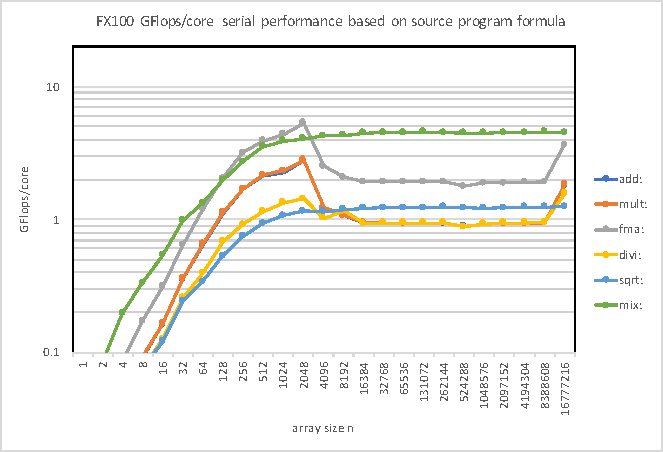
\includegraphics[width=0.45\textwidth]{figs/workload-user.pdf}
%	\caption{workload-user}
%	\label{fig:workload-user}
%	\end{figure}
\begin{figure}[tb]
%\begin{minipage}{0.49\hsize}
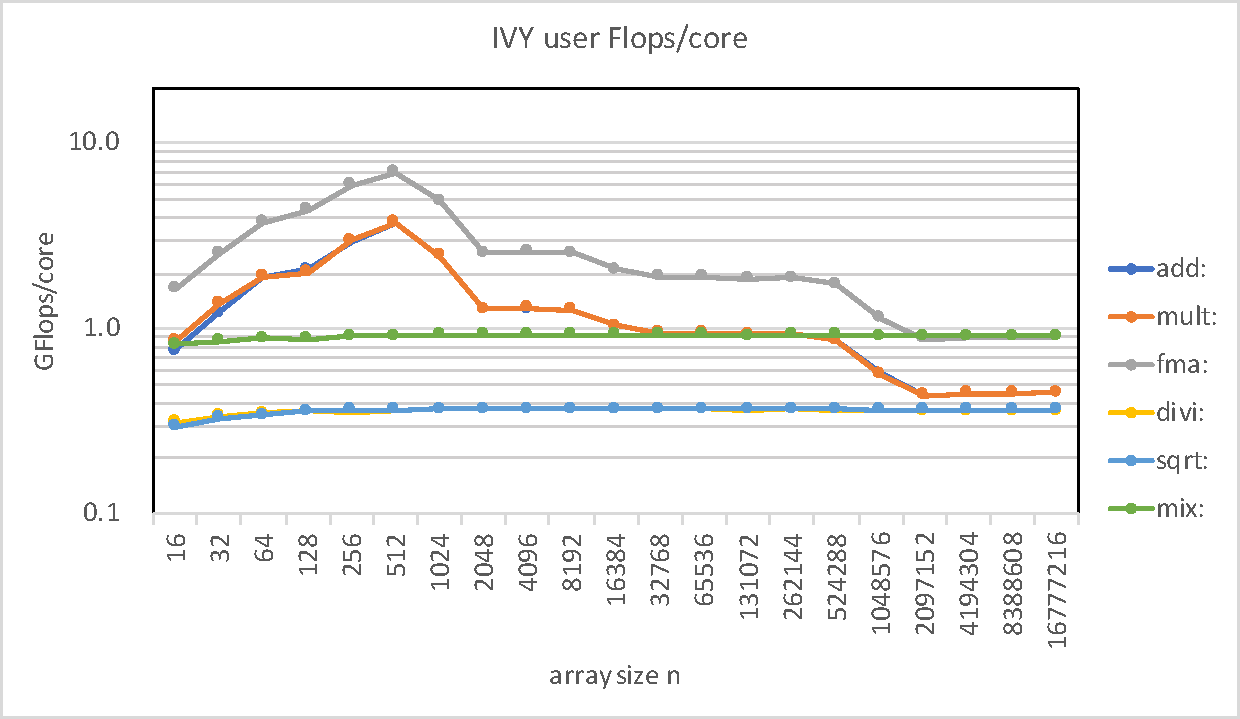
\includegraphics[width=0.5\textwidth]{figs/workload-ivy-user.pdf}
\caption{User perspective workload and performance}
\label{fig:workload-user}
\end{figure}
%\end{minipage}
\begin{figure}[tb]
%\begin{minipage}{0.49\hsize}
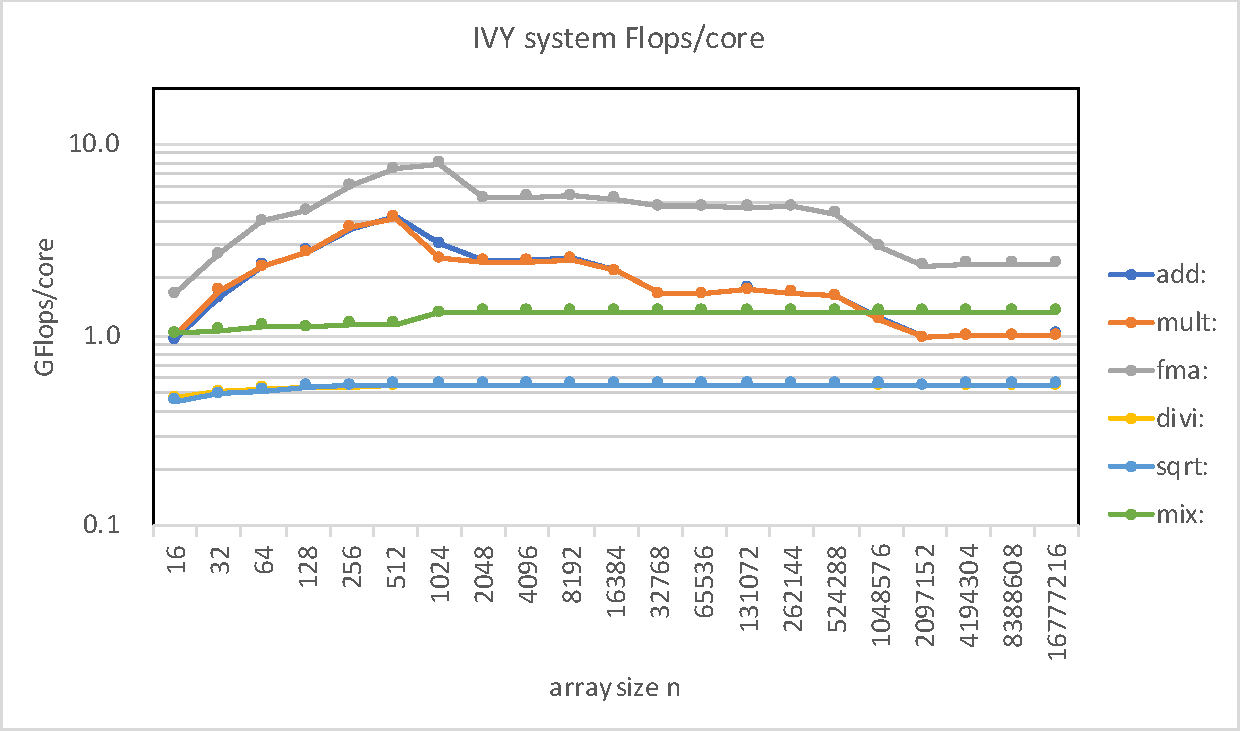
\includegraphics[width=0.5\textwidth]{figs/workload-ivy-system.pdf}
\caption{System perspective workload and performance}
\label{fig:workload-system}
%\end{minipage}
\end{figure}
%
\begin{figure}[tb]
%\begin{minipage}{0.49\hsize}
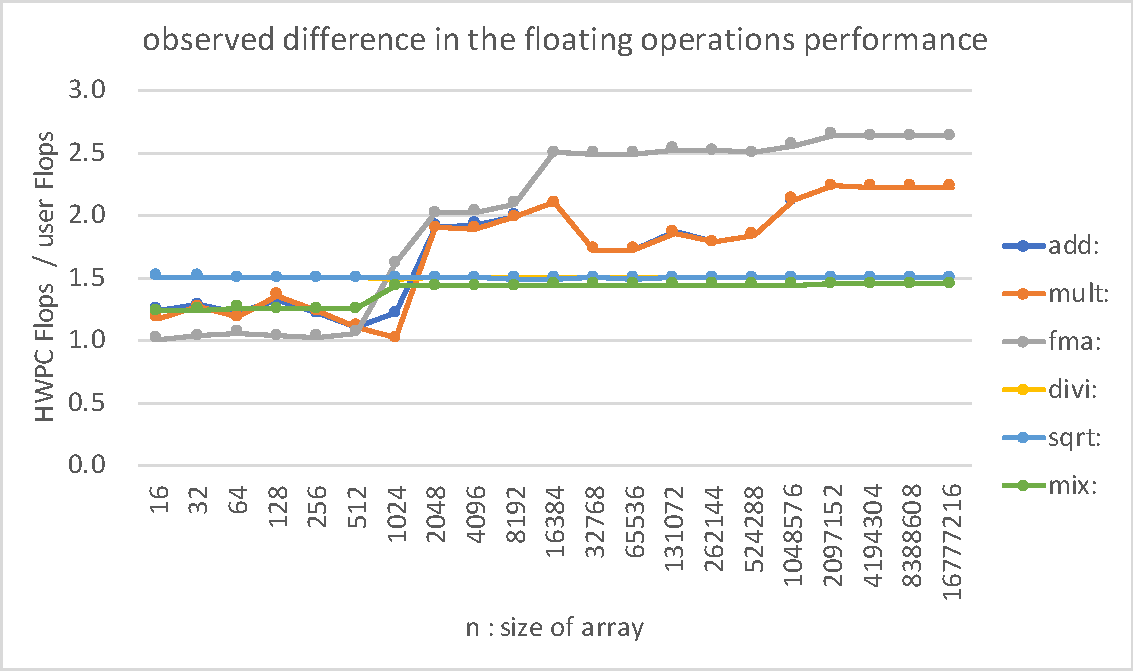
\includegraphics[width=0.5\textwidth]{figs/workload-ivy-difference.pdf}
\caption{Difference between the workloads}
\label{fig:workload-difference}
%\end{minipage}
\end{figure}

This simple example clearly indicates that the performance evaluation of
scientific applications on HPC systems must be associated with a clear
definition of workload. The example also suggests that, if conditions allow,
the evaluation should be conducted for both user and system perspectives.
A detailed analysis of a similar example is given in section
\ref{subsection:basic-kernels}.

%%
\section{Performance Monitoring Library}
\label{section:PMlib}

%
\subsection {Overview of PMlib}
PMlib is an open source library for monitoring the performance of scientific
applications and is able to measure the listed types of workload discussed
in the previous section, i.e. arithmetic, application, and HWPC workloads.
Users can insert start/stop API statements provided in the source code.
Each measurement section has minimal properties such as name, type of operation,
exclusiveness, and workload value.
The reports from PMlib is classified into threads, processes, and sections
depending on the controlling environment variable.

%
\subsection{PMlib API}
%\label{subsection:PMlib-API}
PMlib provides APIs for C++ and Fortran programs.
There are only a small number of APIs which must be called from applications.
C++ APIs are shown in Table~\ref{tab:PMlib-API}. 

\begin{table}[tb]
%\tiny %\scriptsize %\footnotesize %\small
\footnotesize
%	\scriptsize
\caption{list of basic APIs provided by PMlib}
\label{tab:PMlib-API}
\begin{tabular}{l|l|l} \hline
C++	& function	&	arguments	\\ \hline \hline
initialize	& initial setup	& number of sections \\ %\hline
setProperties	& set sections property	& label, type, exclusiveness \\ %\hline
start	& start of section	& label \\ %\hline
stop	& end of section	& label, arithmetic workload \\ %\hline
print	& basic report	& filename, comments, sort order	\\ %\hline \hline
printDetail	& per process report	& filename, legend, sort order	\\ %\hline
\end{tabular}
\end{table}

Fortran APIs follow the similar naming convention,
i.e. f\_pm\_\{{\footnotesize\it{C++API\_name}}\},
The following is an example Fortran program calling PMlib APIs.

%	\begin{lstlisting}[caption={calling PMlib in Fortran program}]
\begin{lstlisting}
program main
	call f_pm_initialize (Nsections)
	call f_pm_setproperties ("section1",icalc,iexcl)
	call f_pm_start ("section1")
	call some_computation (fops)
	call f_pm_stop ("section1",fops,0)
	call f_pm_print ("",0)
	call f_pm_printdetail ("",0,0)
end
\end{lstlisting}

%
\subsection{Choosing workload type}
\label{subsection:Choosing-workload-type}

The choice of the workload is made by a
run-time environment variable HWPC\_CHOOSER
which can take one of the following values.
\begin{quote}
\begin{small}
%	\begin{verbatim}
FLOPS\textbar BANDWIDTH\textbar VECTOR\textbar CACHE\textbar CYCLE%
\textbar user
%	\end{verbatim}
\end{small}
\end{quote}

If the arithmetic workload is measured,
The number of arithmetic operations or the formula defining the workload
must be provided to PMlib API as user argument.
PMlib accumulates the workload per section sandwiched by start and stop APIs.
In practice, counting the number of arithmetic operations in the application
source code can be a non-trivial task, and automating such a task is desirable.
%
To automate the counting task for Fortran applications, we can utilize
the related research~\cite{Hoshimoto:2015},~\cite{ccaebt:HPCAsia2018}
to let the parser program analyze the Fortran source code
and produce JSON intermediate reports showing the arithmetic operations counts.
Then, a second filter can be used to produce the partial Fortran source program
including call statements for PMlib API with provisioned arguments.
%	{\color{blue} Remark. This second filter is under development as of this paper.  }
Fig.~\ref{fig:ccaebt4PMlib} shows the schematic view to accomplish this flow.

\begin{figure}[tb]
\centering
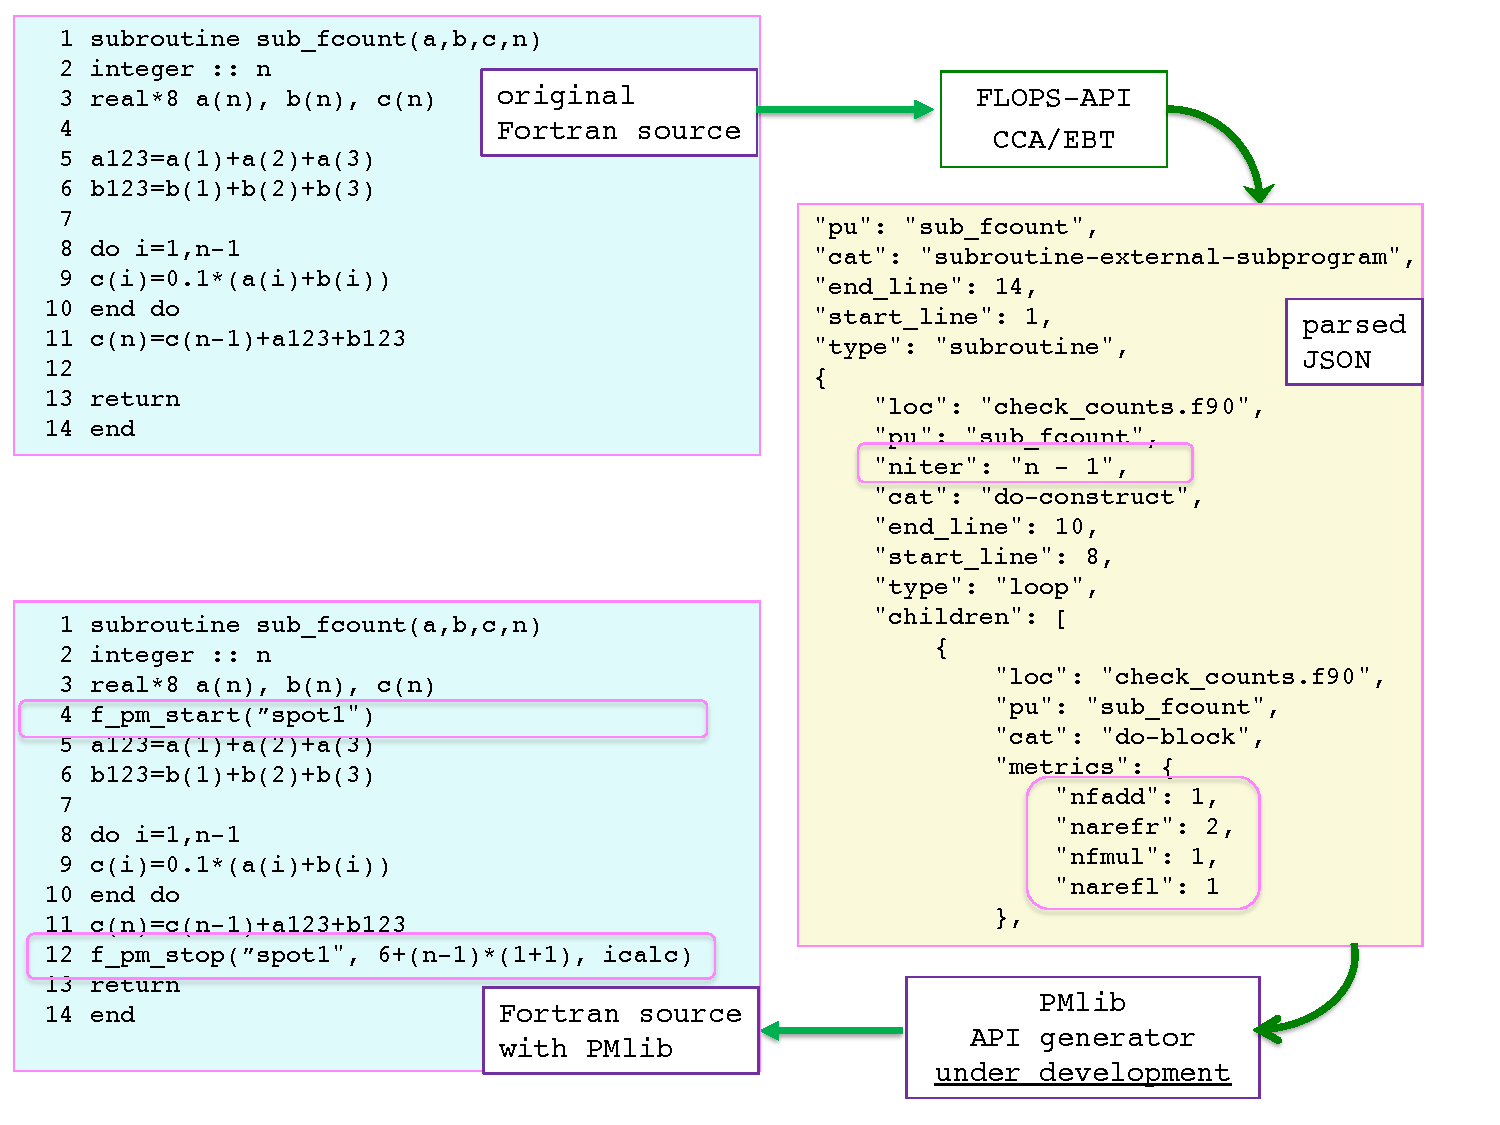
\includegraphics[width=0.5\textwidth]{figs/ccaebt4PMlib.pdf}
\caption{Counting the operation with ccaebt parser program}
\label{fig:ccaebt4PMlib}
\end{figure}

If the HWPC workload is measured,
PMlib internally utilizes PAPI low-level APIs to access HWPC event statistics.
PAPI has its own event mnemonics for each type of processor,
and choosing a set of native PAPI events can be troublesome.
For instance, the standard output from $ papi\_native\_avail $ command on a
Skylake server produces 5000+ lines.
PMlib detects the type of processor,
chooses the appropriate native PAPI event sets
and translates the raw event statistics into the desired
performance category according to HWPC\_CHOOSER.
The user given operation count arguments are discarded in HWPC mode.
PMlib preserves the source code portability in both user mode and HWPC mode.

\subsection{High-resolution timer available to PMlib}
PMlib utilizes the Linux standard timer gettimeofday() by default.
It also has the installation option to utilize
a system specific high-resolution low overhead timer if such timer is
available on the platform.
Fig.~\ref{fig:precise-timer} shows a comparison of a standard timer and
the high-resolution timer on the two HPC systems highlighted in the
previous section.
PMlib has a provision to use them as an installation option.
\begin{figure}[tb]
\centering
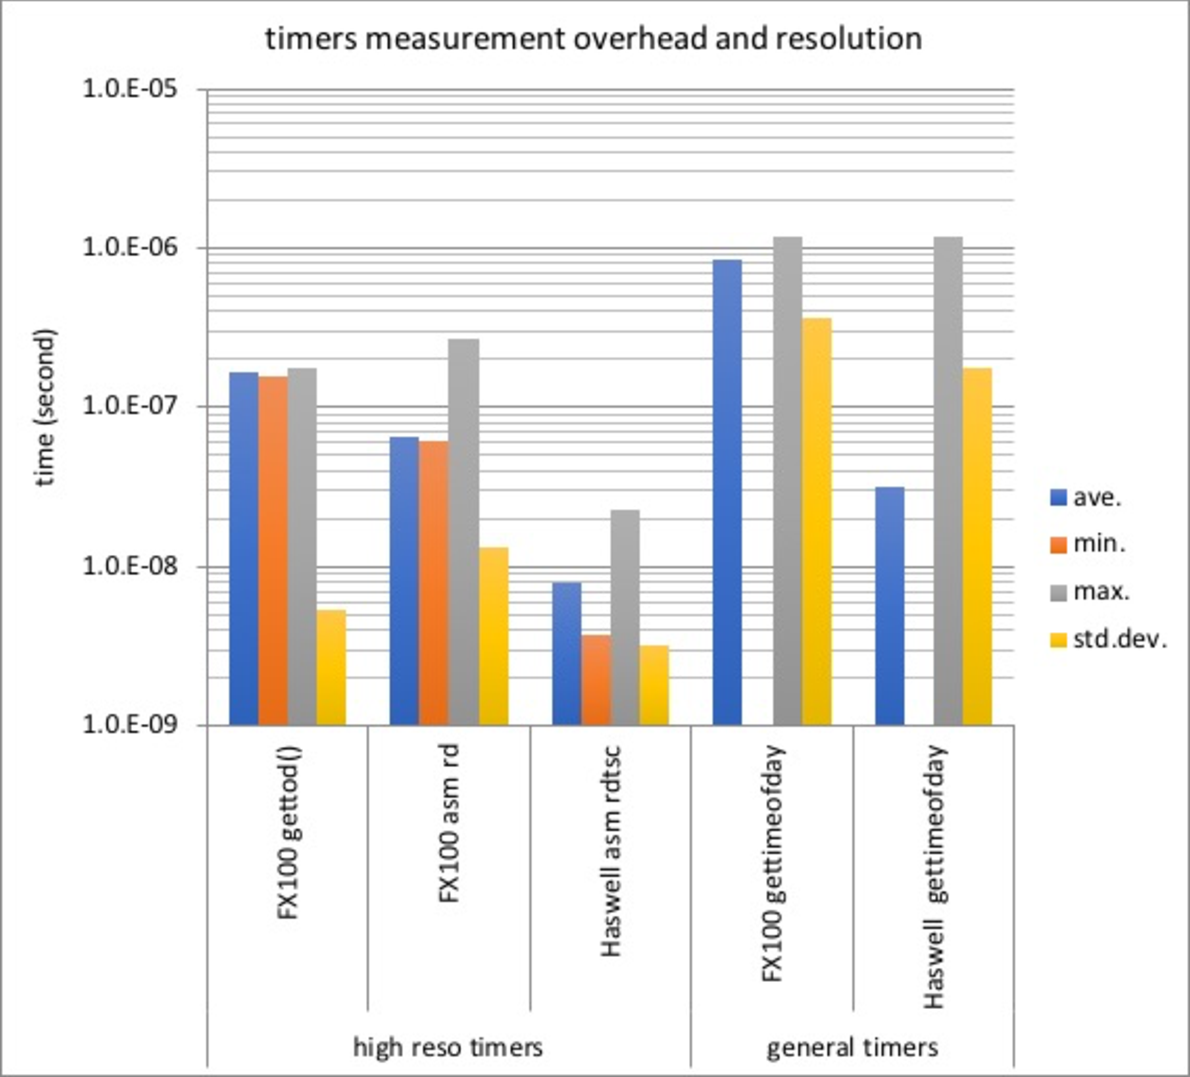
\includegraphics[width=0.45\textwidth]{figs/precise-timer.pdf}
\caption{general timer and precise timer}
\label{fig:precise-timer}
\end{figure}

\subsection{Output information}
\label{subsection:PMlib-output-information}
The default output information from PMlib is a blocked text report based on
the time-averaged performance statistics.
PMlib is also able to produce the
Open Trace Format (OTF)~\cite{Knupfer:2006},~\cite{OTF:webpage-public}
tracing files that may contain the shorter interval statistics for visualization.
%
%	In future papers, we may include TRAiL contents
%
%	Web browser visualization tool TRAiL~\cite{trail}~.%
%	\begin{figure}[tb]
%	\centering
%	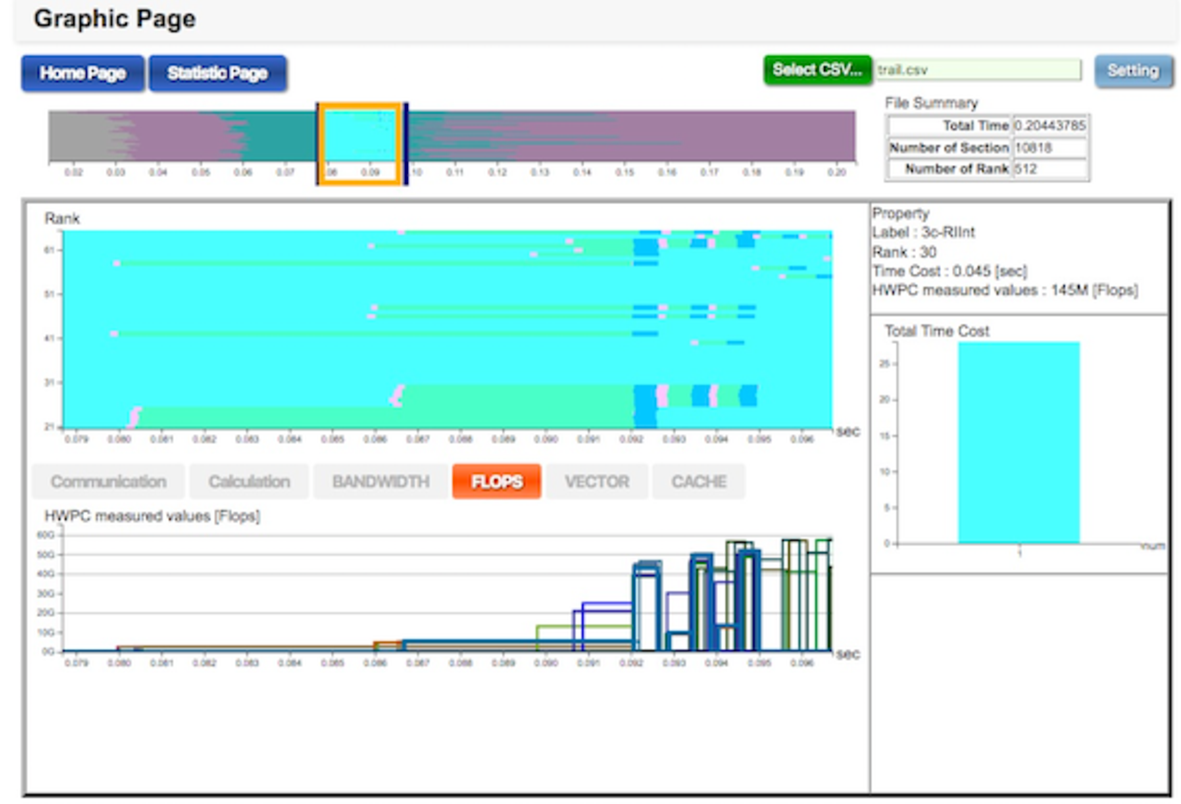
\includegraphics[width=0.45\textwidth]{figs/TRAiL-small.pdf}
%	\caption{tracing visualization using PMlib and TRAiL}
%	\label{fig:TRAiL}
%	\end{figure}


\subsection{Other performance evaluation tools and related research}
\label{subsection:related-research}
Numerous tools have been developed to evaluate the performance of HPC systems.
In general, open source tools are designed to be portable.
Their functionalities are distinct and in many cases, multiple tools
are used in sequence to obtain the desired performance information.
These tools are classified as either sampling or tracing tools and they each have different overheads.
Commercial vendor tools are used for many HPC systems.
They are best used for specific processor types.
HPC systems vendors also supply performance evaluation tools
that are native to their systems.
They are integrated into systems and are easy to use in general,
but availability is limited to only the vendor's HPC systems.

Some of the commonly used tools are listed below.
In the open source category:
\begin{itemize}
	\item Scalasca \cite{Scalasca:2017},\cite{Scalasca:2010}
			: trace generation, Score-P infrastructure
	\item Extrae \cite{Extrae:webpage} :  trace generation
	\item PAPI \cite{PAPI:5.6} : API to access HWPC
	\item Linux perf tools : API to access HWPC
\end{itemize}
In the commercial vendor category:
\begin{itemize}
		\item Intel VTune \cite{Intel:VTune} : Intel processors
		\item PGI Profiler \cite{PGI:Profiler} : X86 and GPU
\end{itemize}
These existing tools all utilize the processor performance information
based on HWPC workload, i.e. system workload.
PMlib appears to be the only tool that enables arithmetic and/or application
workload evaluation.

%%
\section{Performance evaluation using PMlib}
\label{section:using-PMlib}

\subsection{Basic kernels and test servers}
\label{subsection:basic-kernels}

Some examples of performance evaluation utilizing PMlib are shown in this section.
The tested programs are the basic kernels composed of
four basic arithmetic operations, square root and reversed distance.
The kernels repeat the same operations with loop length hidden to the compiler.
%
The Fortran source of these kernels is shown below.
%	\begin{lstlisting}[caption={basic kernels (partial list)}]
\begin{lstlisting}
subroutine sub_add(a,b,c,n)
	do i=1,n
	c(i)=a(i)+b(i)
	end do
subroutine sub_mult(a,b,c,n)
	do i=1,n
	c(i)=a(i)*b(i)
	end do
subroutine sub_fma(a,b,c,d,n)
	do i=1,n
	c(i)=a(i)+b(i)*d
	end do
subroutine sub_divide(a,b,c,n)
	do i=1,n
	c(i)=b(i)/a(i)
	end do
subroutine sub_sqrt(a,b,c,n)
	do i=1,n
	c(i)=sqrt(a(i))
	end do
subroutine sub_mix(a,b,c,n)
	do i=1,n
	c(i)=1.0/sqrt(a(i)**2+b(i)**2)
	end do
\end{lstlisting}

The choice of data precision, either double or single, is made at compile time,
and the default optimization is done by the compilers.
The intent is to exploit pipelined SIMD operations on the measuring systems.
The copies of the same kernel are run on all cores of the processor.
The kernels are called many times.  After the calling overhead is subtracted,
the average elapsed time including the do loop overhead cost is obtained.


The servers used for the tests are:
\begin{itemize}
{
%	\setlength{\itemsep}{-5pt}
%	\setlength{\topsep}{2mm}
\item SGI Intel Ivybridge server
\item SGI Intel Skylake server
\item Fujitsu prime HPC FX100
}
\end{itemize}
Their processor specifications and the major performance specifications
are listed in Table~\ref{tab:server-config}.

\newif\ifTwoservers
\newif\ifThreeservers
\Twoserversfalse
\Threeserverstrue
%\tiny
%\scriptsize
%\footnotesize
%\small
\begin{table}[tb]
\scriptsize
\caption{server configuration and hardware specification}
\label{tab:server-config}
\footnotesize

\ifTwoservers
\begin{tabular}{l|c|c} \hline
\scriptsize
system			&	FX100		&	Skylake	\\ \hline
CPU				&	SPARC64 XIfx	&	Gold 6148	\\ \hline
core GHz		&	1.975		&	2.4	\\ \hline
core Gflops		&	31.6		&	〜30	\\ \hline
\#cores/cpu*	&	16			&	20	\\ \hline
L1\$ size(D,I)	&	64KB, 64KB	&	32KB, 32KB	\\ \hline
L1D\$ BW GB/s	&	140/R+70/W	&	154/R + 77/W	\\ \hline
\$ Linesize 	&	256B		&	64B	\\ \hline
L2\$ size		&	-			&	1MB	\\ \hline
L2\$ BW GB/s/c	&	-		&	154 ( ~70)	\\ \hline
LL\$ size		&	12MB		&	28MB(1.4MB/c)	\\ \hline
LL\$ BW GB/s/c	&	70/R+35/W	&	77 ( ~43)	\\ \hline
Memory			&	HMC(8x16Ls)	&	DDR4-2666	\\ \hline
Mem GB/s/[CMGcpu]	&	120/R+120/W	&	128	\\ \hline
\multicolumn{3}{l}{\scriptsize\hspace{5mm} remark. cpu* indicates processor or CMG }\\
\end{tabular}
\fi
\ifThreeservers
\begin{tabular}{l|c|c|c} \hline
\scriptsize
Symbol			&	FX100		&	SKY		&	IVY \\ \hline
Platform		&	FX100		&	Skylake & Ivybridge\\ \hline
CPU				&	SPARC64 XIfx	&	Gold 6148	&	E5-4620v2	\\ \hline
core GHz		&	1.975		&	2.4	&	2.6 \\ \hline
core Gflops		&	31.6		&	~30	\\ \hline
\#cores/cpu*	&	16			&	20	&	8	\\ \hline
L1\$ size(D,I)	&	64KB, 64KB	&	32KB, 32KB	\\ \hline
L1D\$ BW GB/s	&	140/R+70/W	&	154/R + 77/W	\\ \hline
\$ Linesize 	&	256B		&	64B	&	64B	\\ \hline
L2\$ size		&	-			&	1MB	&	256KB	\\ \hline
L2\$ BW GB/s/c	&	-			&	154 ( ~70)	\\ \hline
LL\$ size		&	12MB		&	28MB	&	20 MB	\\ \hline
LL\$ BW GB/s/c	&	70/R+35/W	&	77 ( ~43)	\\ \hline
Memory			&	HMC(8x16Ls)	&	DDR4-2666	& DDR3-1600	\\ \hline
Mem GB/s/cpu*	&	120/R+120/W	&	128	\\ \hline
\multicolumn{4}{l}{\scriptsize\hspace{5mm} remark. cpu* indicates processor or CMG }\\
\end{tabular}
\fi
\end{table}


\subsection{Kernel performance on FX100 in long loops}
\label{subsection:long-kernels-fx100}
%
\if 0
% We must cut the following important remarks because of the short space.
% Noise elimination can be a section volume!
% It is not a simple task to suppress or eliminate the noise from measurements.
% 
% OS noise.
% Various jitter effects cause delay.
% Shared noise.
% Typical HPC systems are simultaneously shared by many users and tend to
% suffer from perturbation influences called noise caused by other processes,
% including the delay caused by shared file systems, networks congestion, etc.
% This perturbation influence is usually more apparent on large scale systems.
% 
% Dynamic effect.
% unexpectable run-time hardware behavior such as out-of-order execution.
% 
% The countermeasure.
% On the user side, noise elimination can be addressed via statistical
% approaches. These include the addition of an outer loop for repeated
% measurement and the filtering of measurements values that fall outside of
% a standard deviation window.
%
% the noise has been removed as explained here...???
\fi
%
Fig.~\ref{fig:fx100-gflops-user-long-R8} shows the 
user performance,i.e. arithmetic performance, of the basic kernels
on FX100 system
for the loop length of
\begin{math}
n=1,2,4,..,2^{24}
\end{math}
.

Fig.~\ref{fig:fx100-gflops-system-long-R8} shows the 
system performance based on the HWPC workload.
The HWPC workload of the floating point operations on FX100 is
recorded as events sorted by SIMD width as below.
%	\begin{figure}[H]
%	\end{figure}
\begin{quote}
\begin{small}
\begin{verbatim}
fpdp1  : "1FLOPS_INSTRUCTIONS";
fpdp2  : "2FLOPS_INSTRUCTIONS";
fpdp4  : "4FLOPS_INSTRUCTIONS";
fpdp8  : "8FLOPS_INSTRUCTIONS";
fpdp16 : "16FLOPS_INSTRUCTIONS";
\end{verbatim}
\end{small}
\end{quote}
The total number of HWPC floating point operations
is calculated as the sum of single precision and double precision operations.
\begin{align}
	\mathrm{W}_{hwpc} & = \mathrm{fpdp1} + 2.0*\mathrm{fpdp2} + 4.0*\mathrm{fpdp4} \nonumber \\
			& + 8.0*\mathrm{fpdp8} + 16.0*\mathrm{fpdp1} 
\end{align}

\begin{figure}[tb]
\centering
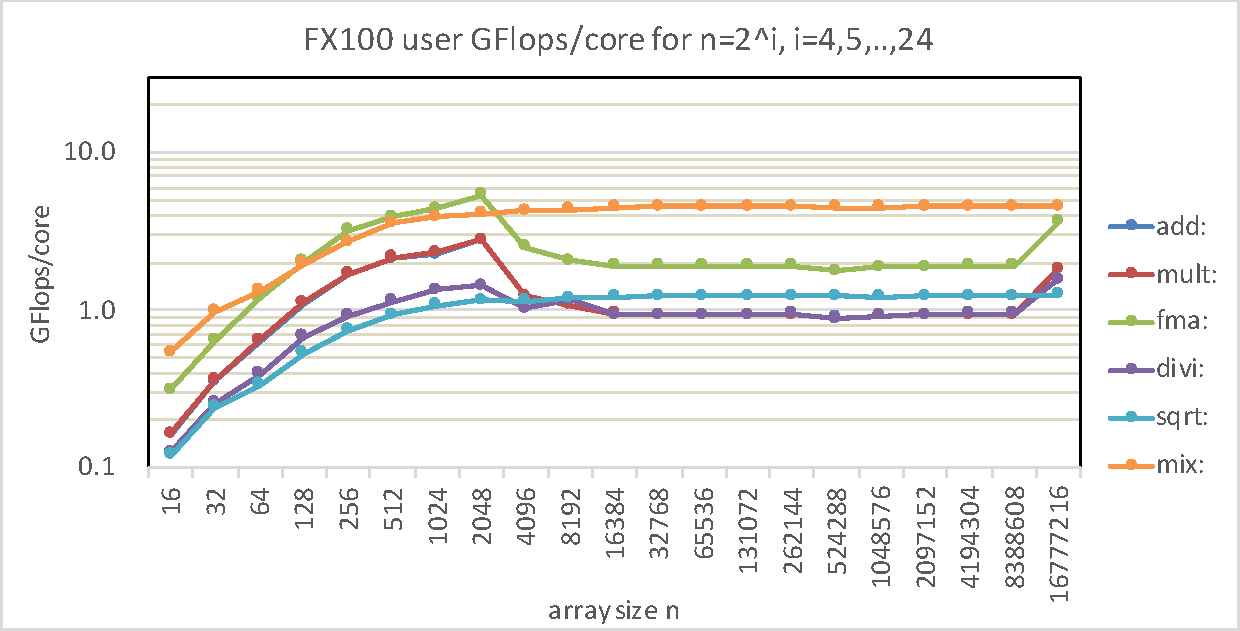
\includegraphics[width=0.45\textwidth]{figs/fx100-gflops-user-long-R8.pdf}
\caption{user performance of FX100 for basic kernels}
\label{fig:fx100-gflops-user-long-R8}
\end{figure}

\begin{figure}[tb]
\centering
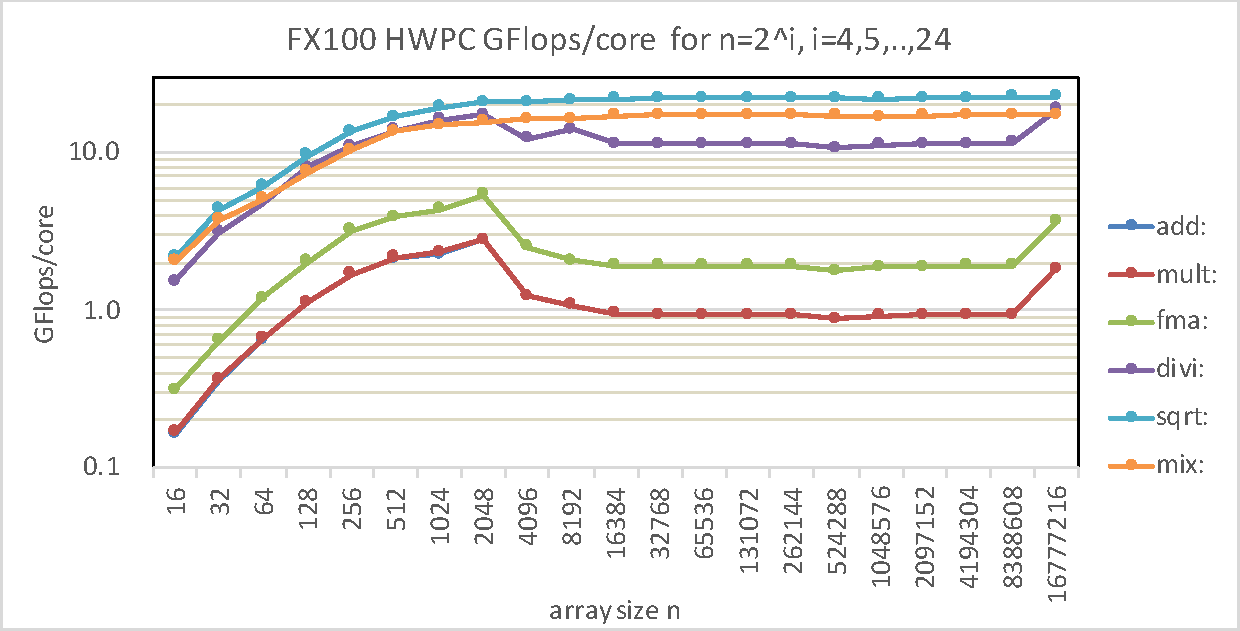
\includegraphics[width=0.45\textwidth]{figs/fx100-gflops-system-long-R8.pdf}
\caption{system performance of FX100 for basic kernels}
\label{fig:fx100-gflops-system-long-R8}
\end{figure}

\begin{figure}[tb]
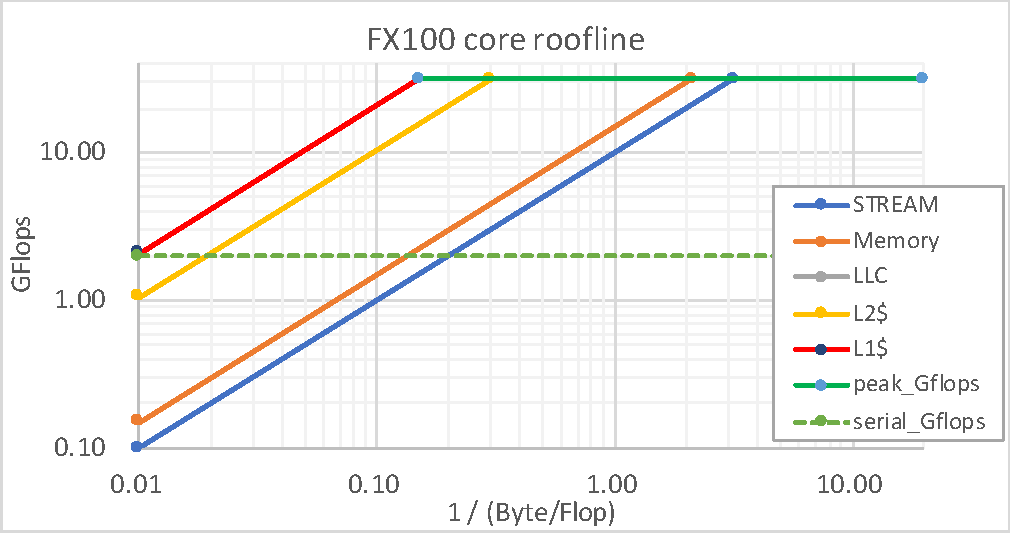
\includegraphics[width=0.45\textwidth]{figs/roofline-fx100.pdf}
\caption{roofline envelop of FX100}
\label{fig:roofline-fx100}
\end{figure}

In both figures,
the performance of add/mult/fma tends to improve with an increase of
the loop length until the L1 cache size limit is reached,
and subsequently drops to the bandwidth constrained performance level
of the next level cache.
This performance tendency for add/mult/fma is consistent with the reports
from other related research investigations.
It can be associated with the roofline~\cite{Williams:2009}
envelop which is shown in Fig.~\ref{fig:roofline-fx100}

The performance of div/sqrt/mix shows quite different tendency, and
their system performance stays much higher than the user performance.

Partial results extracted from PMlib HWPC report are shown
in Table~\ref{tab:PMlib-report-HWPC}.
%
\begin{table}[bt]
\centering
\caption{PMlib HWPC events for HWPC\_CHOOSER}
\label{tab:PMlib-report-HWPC}
\scriptsize %\tiny %\scriptsize %\footnotesize %\small
% \input{figs/stdout.PMlib-report-HWPC.txt}
%
\begin{tabular}{l|c|c|c|c|c|c}
\\ \hline
kernel  	& 1fp.ins  & 2fp.ins  & 4fp.ins  & 8fp.ins  & 16fp.ins  & vector\%
\\ \hline
sub\_add  	& 1.90e+2  & 2.60e+2  & 5.12e+5  & 0.00e+0  & 0.0e+0  & 1.0e+2
\\
sub\_fma  	& 2.00e+2  & 2.60e+2  & 0.00e+0  & 5.12e+5  & 0.0e+0  & 1.0e+2
\\
sub\_divide	& 1.90e+2  & 2.60e+2  & 1.02e+6  & 2.56e+6  & 0.0e+0  & 1.0e+2
\\ \hline
\end{tabular}
%

\end{table}
%
The environment variable HWPC\_CHOOSER explained in
\ref{subsection:Choosing-workload-type} is set to VECTOR in this case,
and the native HWPC events related with vectorization are sorted and reported.

According to the report,
the number of required operations for division is almost an order of magnitude
more than that for addition, even though their arithmetic workload
is the same.
Compiler optimization transforms
a division arithmetic statement into a series of reciprocal
approximation and multiply-add instructions, rather than issuing
a simple division instruction. They take advantage of pipelined sequence of
SIMD instructions and maintain high flop/byte ratio.
So the apparent system performance of this operation becomes very high,
but the actual user performance is much lower, almost the same as
add/mult in this case. In fact, divide kernel runs much slower than add/mult,
if not pipelined at all.
The comparison of system/user performance ratio is shown in
Table~\ref{tab:ratio-system-user-fx100}.
\begin{table}[bt]
\centering
\caption{ratio of system/user performance of FX100 for basic kernels}
\label{tab:ratio-system-user-fx100}
\begin{tabular}{l|c|c|c|c|c|c} \hline
type &	add	&	mult &	fma &	div &	sqrt &	mix \\ \hline
ratio &	1.0 &	1.0 &	1.0 &	12.0 &	18.0 &	38.0 \\ \hline 	
\end{tabular}
\end{table}
%
The numbers in the table can be
directly obtained from HWPC\_CHOOSER=FLOPS setting.
%	This causes the difference between 
%	Figure~\ref{fig:fx100-gflops-user-long-R8}
%	and
%	Figure~\ref{fig:fx100-gflops-system-long-R8}
%	.
Without having to read the assembly code generated by the compiler,
users can capture some idea from the statistics of PMlib HWPC report.

The reason for the system performance curves of div/sqrt/mix
not having the drop near the L1 cache size limit
is explained by the high computational density which hides the
data supply bandwidth.


\subsection{Kernel performance on FX100 in short loops}
\label{subsection:short-kernels-fx100}

We now take a closer look at short loop region where
the overhead to process the loop set-up and update cannot be neglected,
and the data access latency affects more compared to long loop region.
%	thus the performance characteristics should be associated with

Fig.~\ref{fig:fx100-gflops-short-R8}
shows the close-up user performance of the same basic kernels for
\begin{math}
n=1,2,3,..,50
\end{math}
.
%
The performance curves do not show the gradual increase. Instead, they
show steep stepping shapes at multiples of a constant interval.
% This is a common observation for systems with processors that support SIMD,
% and the interval corresponds to the data width of the SIMD instructions.
Similar stepping behavior of the performance
is observed on other HPC systems with SIMD supporting processors as well,
and its pattern interval corresponds to the data width of the SIMD instructions.

FX100 can utilize 256-bit wide data access and arithmetic SIMD instructions.
In double precision arithmetic the resulting widest interval is
\begin{math}
256 / 64 = 4
\end{math}
.
So the performance is expected to be efficient at $ n=4,8,12,\cdots $.
Fig.~\ref{fig:fx100-gflops-short-R8} verifies such expectation.
It highlights the fact that
program coding practices that maintain the loop length as a multiple of
the SIMD width has a significant impact on the user performance
in short loop computation.
\begin{figure}[tb]
\centering
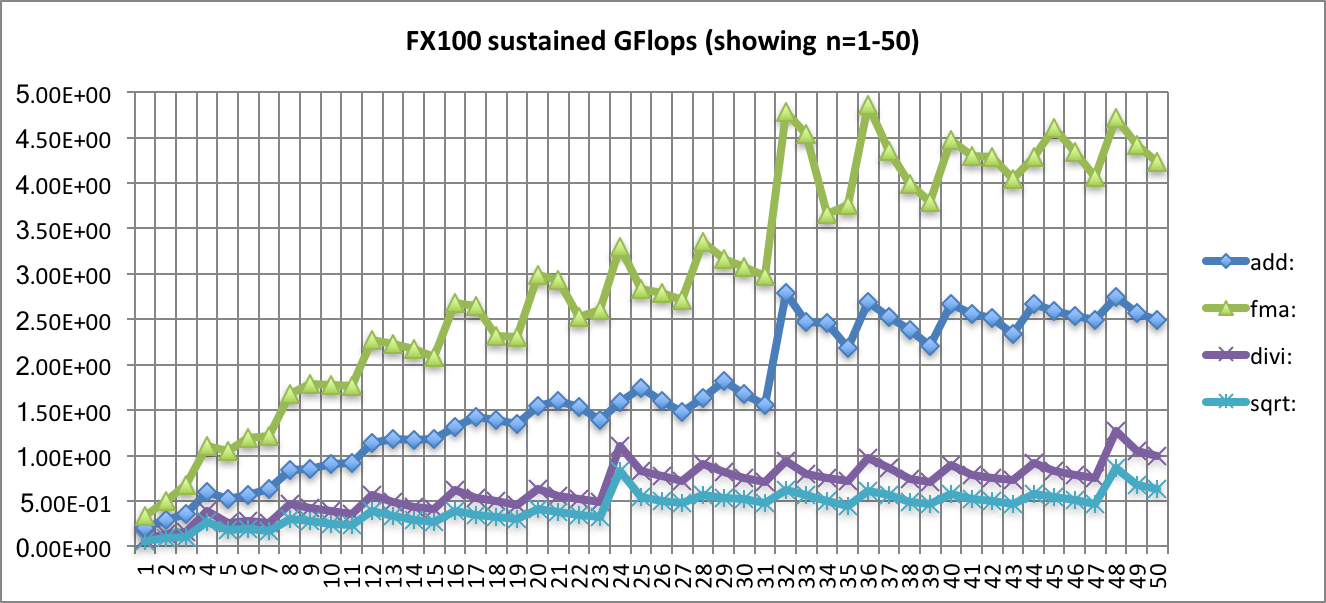
\includegraphics[width=0.45\textwidth]{figs/fx100-gflops-short-R8.pdf}
\caption{FX100 user performance close up}
\label{fig:fx100-gflops-short-R8}
\end{figure}

For single precision, the interval becomes
\begin{math}
256 / 32 = 8
\end{math}
, and the performance impact is even stronger as seen in
Fig.~\ref{fig:fx100-gflops-short-R4} for FX100.
\begin{figure}[tb]
\centering
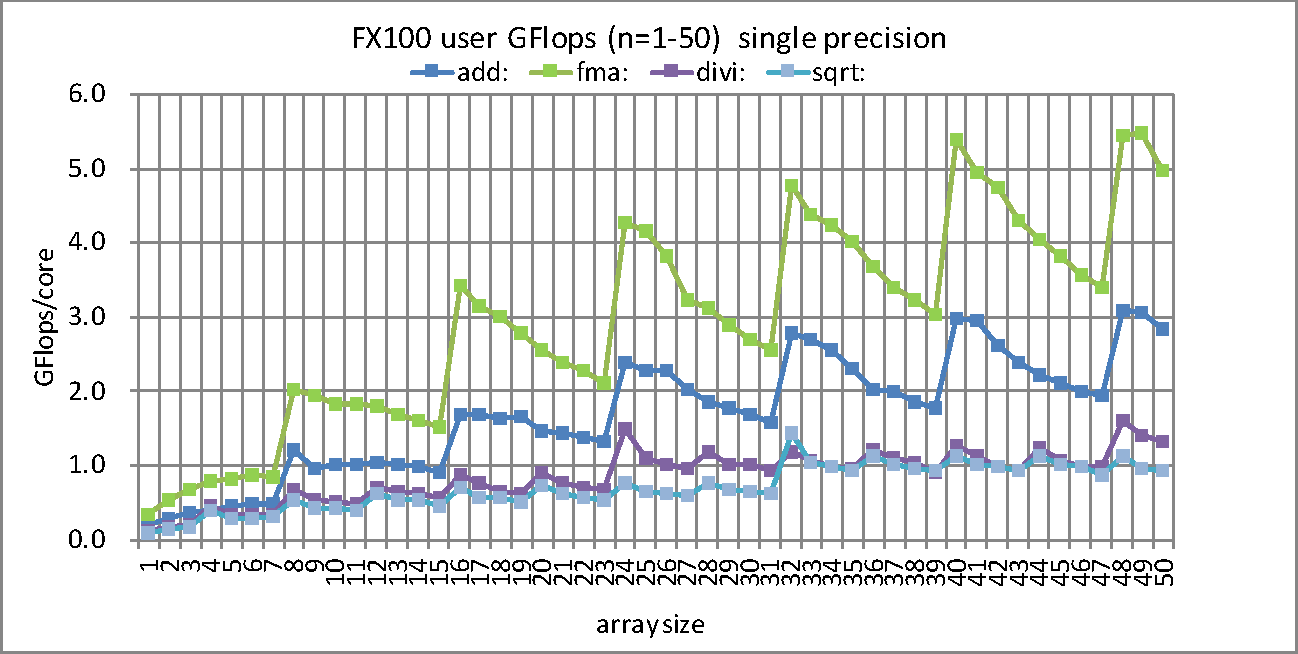
\includegraphics[width=0.45\textwidth]{figs/fx100-gflops-short-R4.pdf}
\caption{FX100 user performance close up for single precision kernels}
\label{fig:fx100-gflops-short-R4}
\end{figure}


\subsection{Kernel performance on SKY in short loops}
\label{subsection:short-kernels-sky}

The performance measurement is also conducted on SKY.
We focus on the short loop region, again.
Fig.~\ref{fig:sky-user-short-R8}
shows the double precision user performance of the same basic kernels on SKY.
The overall line shapes appear similar to that of FX100,
i.e.  stepping shapes at $ n=4,8,12,\cdots $.
Since SKY supports 512-bit wide SIMD instructions called avx512,
the stepping interval is expected to be
\begin{math}
512 / 64 = 8
\end{math}
.
Checking the PMlib HWPC reports tells that the kernels are executed
mostly using 256-bit wide SIMD instructions, not 512-bit.
Further check into the assembly code matched this report.
Knowing this, a compiler option is added to force producing 512-bit instructions.
The revised test results are shown in
Fig.~\ref{fig:sky-user-short-R8-avx512}.
Steppings are now observed at $ n=8,16,\cdots $, but in different shapes.
This revised performance obviously reflects the effect of compiler optimization.

\begin{figure}[tb]
\centering
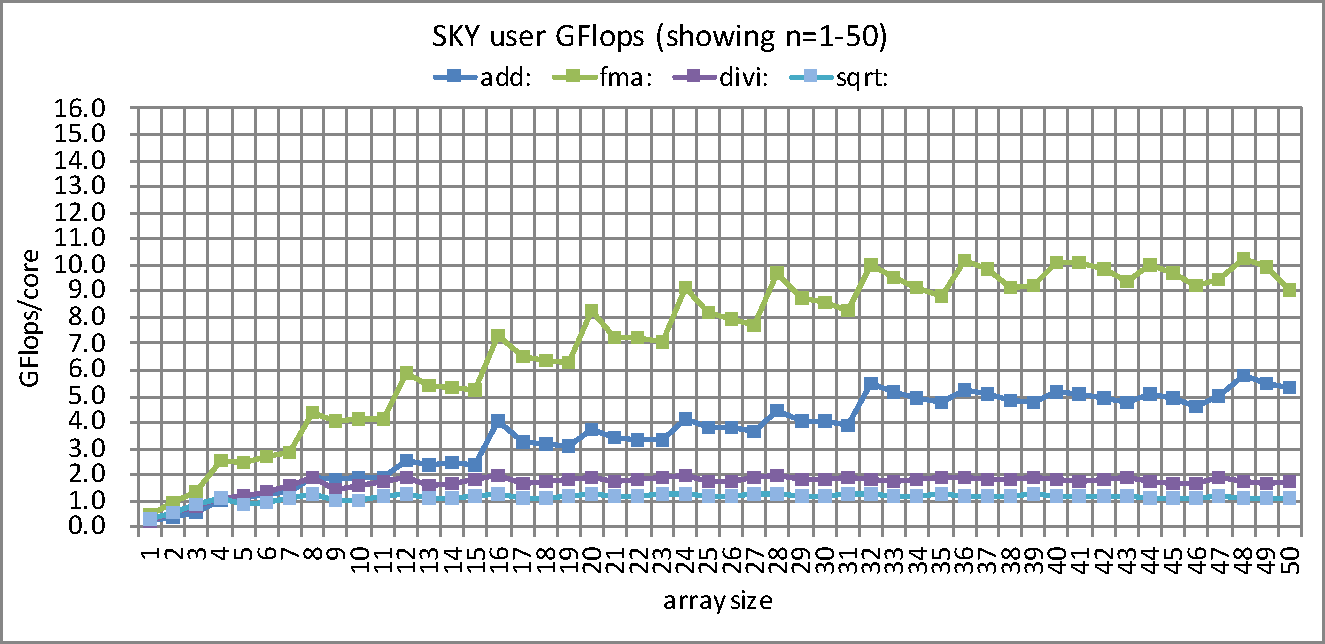
\includegraphics[width=0.45\textwidth]{figs/sky-user-short-R8.pdf}
\caption{SKY user performance close up}
\label{fig:sky-user-short-R8}
\end{figure}
%
\begin{figure}[tb]
\centering
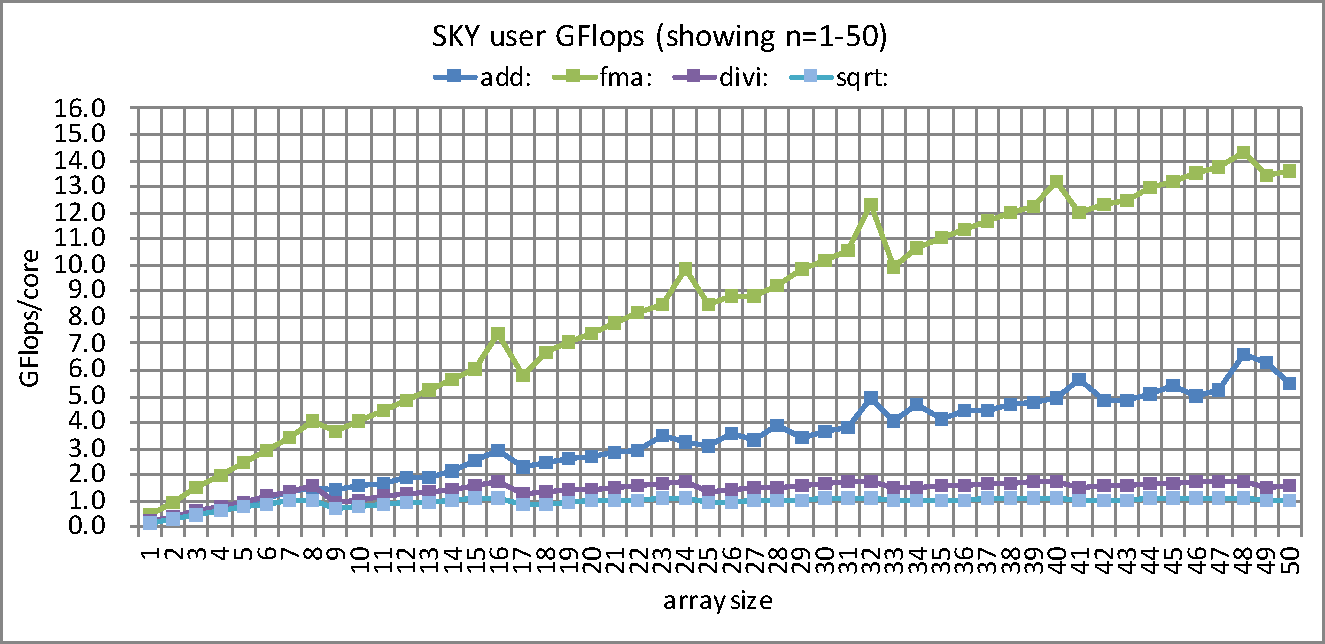
\includegraphics[width=0.45\textwidth]{figs/sky-user-short-R8-avx512.pdf}
\caption{SKY user performance close up forcing 512-bit SIMD}
\label{fig:sky-user-short-R8-avx512}
\end{figure}
%
% \if 0
% Well, no space again. I will delete this interesting picture...
% The single precision user performance is similar as shown in
% fig.~\ref{fig:sky-user-short-R4} .
% \begin{figure}[tb]
% \centering
% 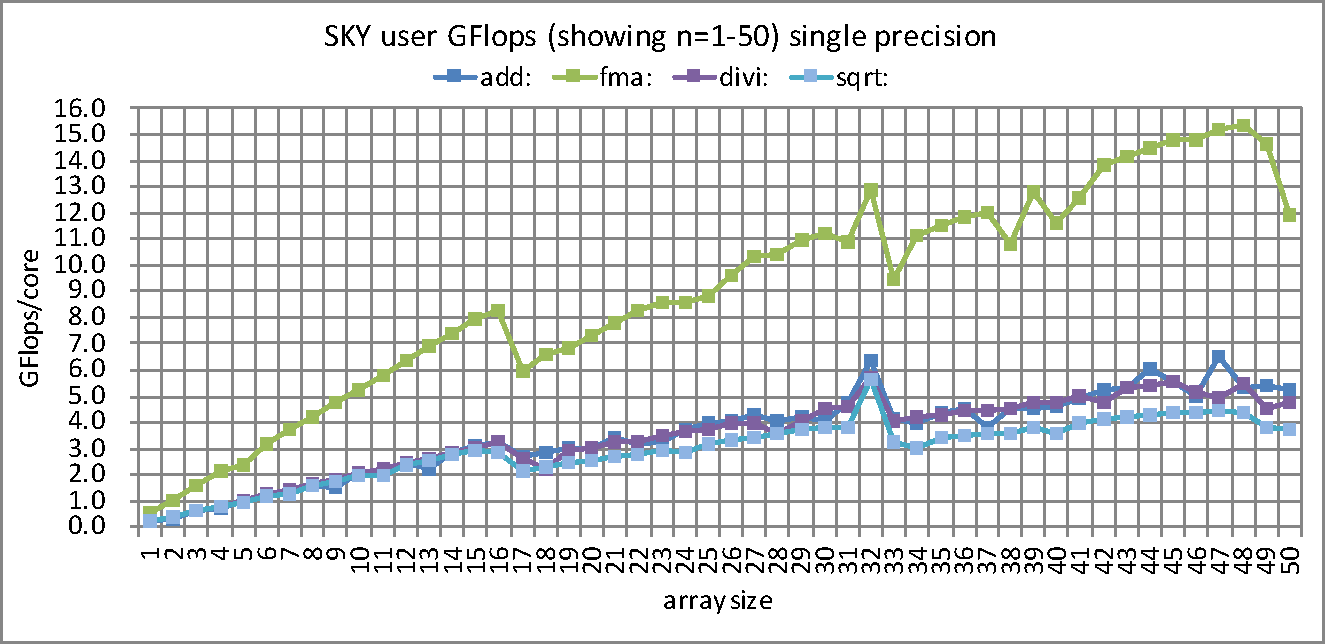
\includegraphics[width=0.45\textwidth]{figs/sky-user-short-R4-avx512.pdf}
% \caption{SKY user performance close up single precision forcing 512-bit SIMD}
% \label{fig:sky-user-short-R4-avx512}
% \end{figure}
%
% \fi
%
% The IVY results are ommited because of paper space.
%	IVY also shows the similar performance characteristics.
%	Fig.~\ref{fig:ivy-gflops-short-R8} shows the user performance
%	of the same basic kernels on IVY. The stepping behavior of SIMD on IVY
%	appears to be less than that of FX100.
%	\begin{figure}[tb]
%	\centering
%	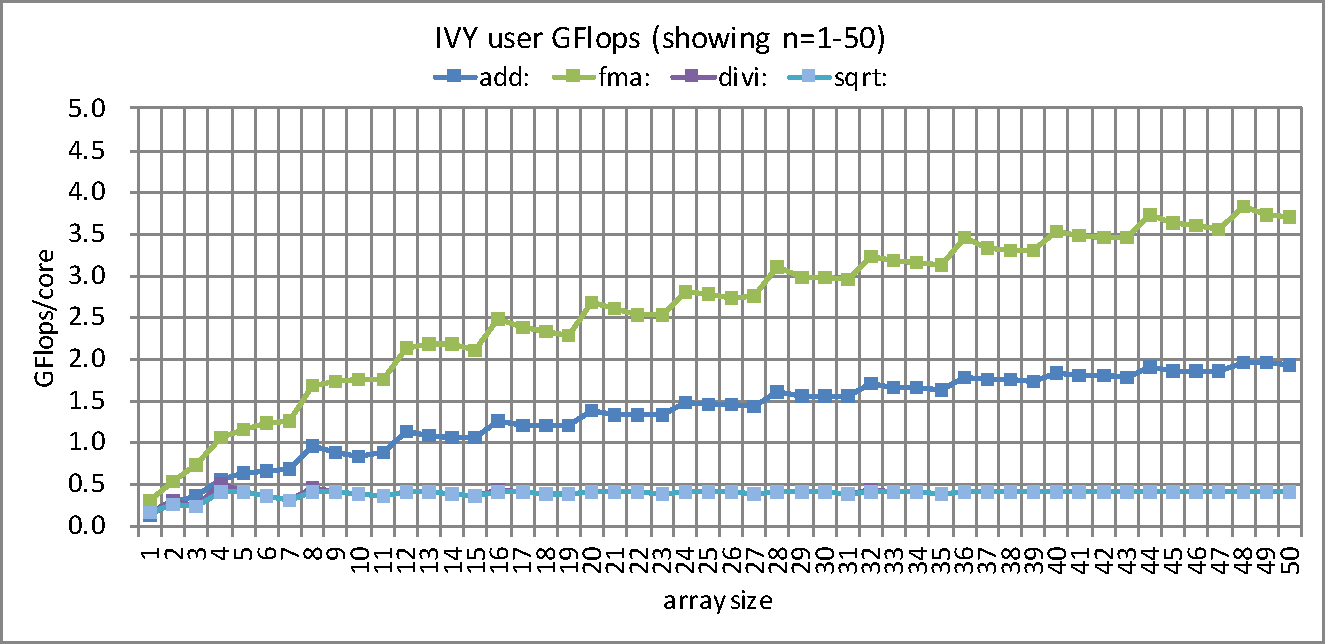
\includegraphics[width=0.45\textwidth]{figs/ivy-gflops-short-R8.pdf}
%	\caption{user performance of IVY for basic kernels}
%	\label{fig:ivy-gflops-short-R8}
%	\end{figure}

\subsection{Future development}
\label{subsection:future-development}
Using PMlib, users are able to obtain various performance information.
In order to reflect the obtained information to the improvement
process of user performance, there can be many approaches going forward.
From PMlib development side,
one approache would be to report the combined information
of user workload and system workload.
If PMlib is able to report the saturated components in the processor hardware
in relationship to the user defined section in the source program,
it maybe a useful index to optimize not only the application source
but also the design of the future hardware.
Further research is needed to harness such feature.

%
% No space. STREAM subsection is omitted.
%
%	\if 0
%	\subsection{STREAM}
%	\label{subsection:STREAM}
%	STREAM benchmark~\cite{stream:1995}
%	has been widely used to measure the memory bandwidth of computer systems.
%	The standard output of this benchmark includes information on the
%	basic arithmetic performance of copy, multiplication, addition,
%	and multiplication\&addition, i.e. arithmetic workload perspective.
%	
%	STREAM HWPC performance shows different characteristics compared to
%	the reported STREAM arithmetic performance. Their performance is influenced by
%	the combined effect of compilers and their optimization options.
%	Although this paper does not intend to provide an exhaustive review of this process,
%	a few points of interest related to the bandwidth are presented.
%	
%	The STREAM Fortran OpenMP result for IVY using 8 threads packed in a CPU
%	is shown first in Fig.~\ref{fig:stream-ivy-1cpux8T}.
%	Then, we compare fig.\ref{fig:stream-ivy-1cpux8T}
%	with
%	Fig.~\ref{fig:stream-ivy-4cpux2T}, 
%	which shows the result using 8 threads scattered over 4 CPUs.
%	
%	The values reported by STREAM for packed thread assignment is better
%	if the streaming-store option is used.
%	%
%	%	% minipage
%	%	\begin{figure}[tb]
%	%	\begin{minipage}{0.48\hsize}
%	%	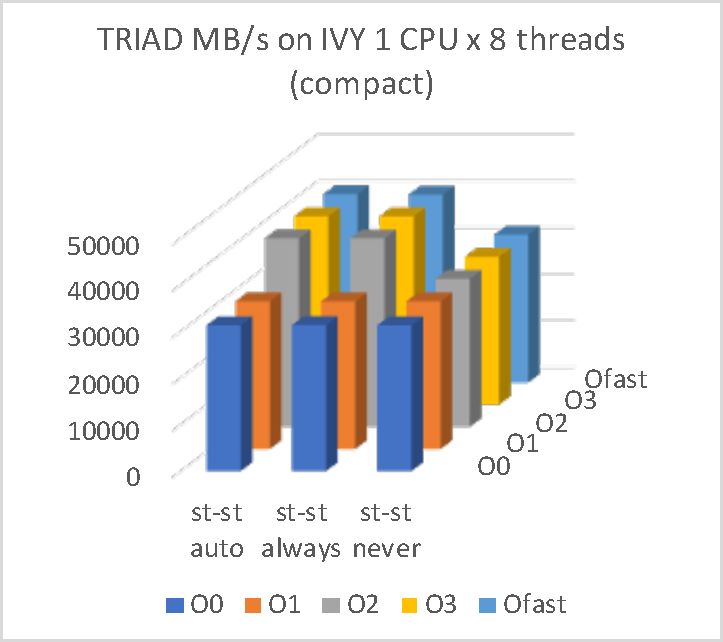
\includegraphics[width=0.98\textwidth]{figs/stream-ivy-1cpux8T.pdf}
%	%	\caption{stream-ivy-1cpux8T}
%	%	\label{fig:stream-ivy-1cpux8T}
%	%	\end{minipage}
%	%	\begin{minipage}{0.48\hsize}
%	%	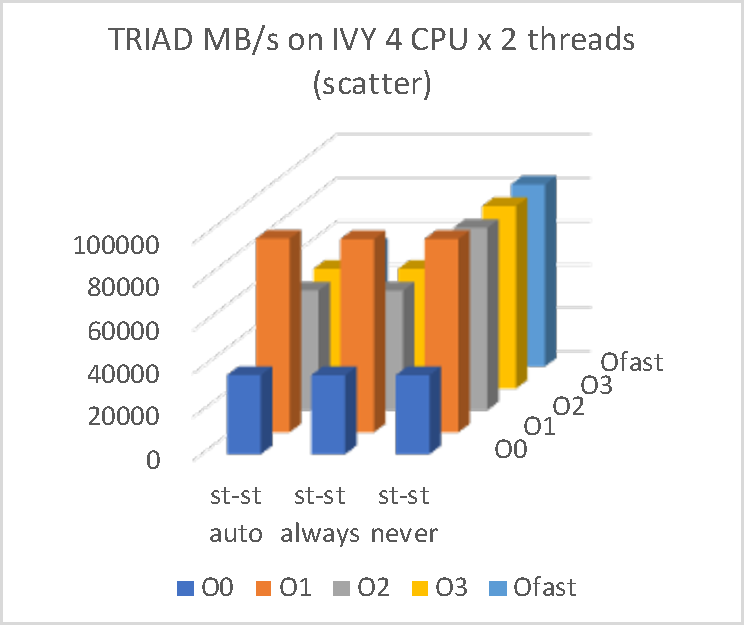
\includegraphics[width=0.98\textwidth]{figs/stream-ivy-4cpux2T.pdf}
%	%	\caption{stream-ivy-4cpux2T}
%	%	\label{fig:stream-ivy-4cpux2T}
%	%	\end{minipage}
%	%	\end{figure}
%	%
%	\begin{figure}[tb]
%	\centering
%	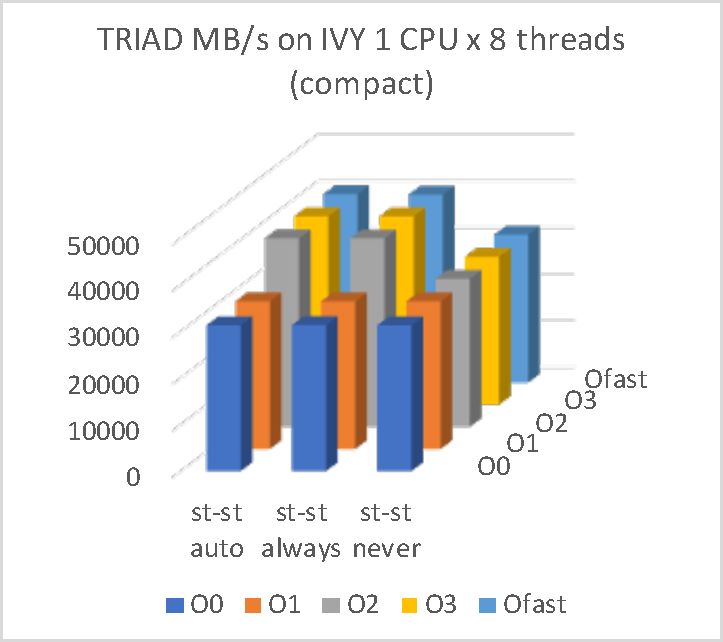
\includegraphics[width=0.45\textwidth]{figs/stream-ivy-1cpux8T.pdf}
%	\caption{Stream-ivy-1cpux8T}
%	\label{fig:stream-ivy-1cpux8T}
%	\end{figure}
%	\begin{figure}[tb]
%	\centering
%	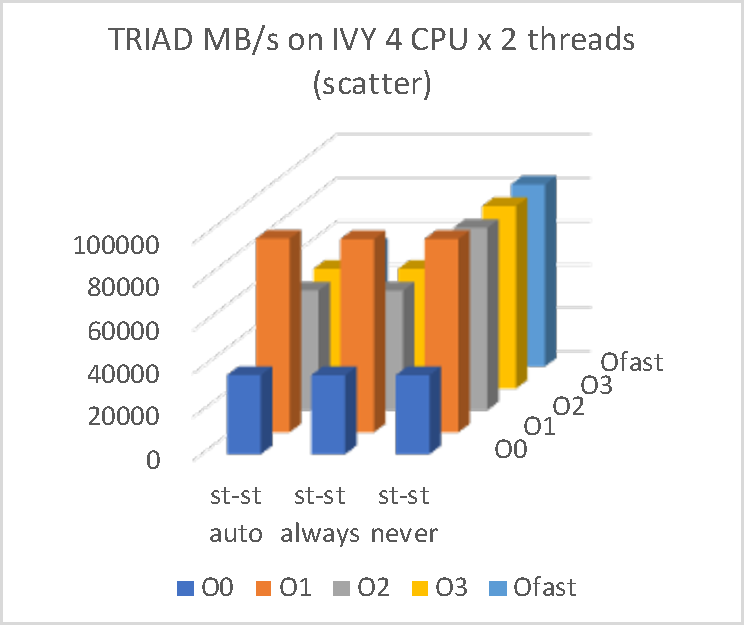
\includegraphics[width=0.45\textwidth]{figs/stream-ivy-4cpux2T.pdf}
%	\caption{Stream-ivy-4cpux2T}
%	\label{fig:stream-ivy-4cpux2T}
%	\end{figure}
%	\fi
%
%%
\section{Conclusion}
In this paper, we discussed the importance of multi-perspective evaluation
to understand the performance characteristics. The difference between
the arithmetic workload coded as the source program and the system workload
executed as machine instructions explains the gap between the user expected
performance and the actually achieved performance on HPC systems.
We presented an open source library called PMlib, which analyzes the behavior
of these workloads.
PMlib provides an avenue for reporting the arithmetic/application workload
as well as the actually executed system workload.
It also provides detailed utilization reports of processor-specific hardware
including the SIMD instruction statistics, the layered cache
hit/miss rate, and the effective memory bandwidth,
which are captured via hardware performance counters through PAPI library.
We could clarify the distinctive behavior by applying the PMlib to a target
program on different hardware architectures, and also verified that PMlib
allows users to conduct synthetic analyses of application performance,
thus enabling the users to obtain useful feedback for further optimizations
and better performance.

\section*{Acknowledgment}
This research used some computational resources of the K computer at the RIKEN Center for Computational Science in Kobe, Japan, and was carried out using the computer resources offered under the category of a general project by the Research Institute for Information Technology, Kyushu University.
%	\section*{References}
\bibliographystyle{jplain}
\bibliography{PMlib}
\end{document}

